\documentclass[preprint]{style}
\pagenumbering{arabic}

\usepackage{paralist}
\usepackage{graphicx}
\usepackage{url}
\usepackage{amsmath}



% This gets rid of the block of whitespace on the first page
\makeatletter
\let\@copyrightspace\relax
\makeatother


\addtolength{\topmargin}{-.07in}
\addtolength{\textheight}{.07in}

%\addtolength{\oddsidemargin}{-0.08in}
%\addtolength{\evensidemargin}{-0.08in}
%\addtolength{\textwidth}{0.08in}



\begin{document}

\title{Medical Concept Extraction}

\numberofauthors{3}
\author{
\alignauthor
Tristan Naumann\\
\affaddr{MIT EECS}
\email{tjn@mit.edu}
\alignauthor
Samantha Ainsley\\
\affaddr{MIT EECS}
\email{ainsley@mit.edu}
\alignauthor
Salman Ahmad\\
\affaddr{MIT EECS}
\email{saahmad@mit.edu}
}

\date{14 December 2012}

\maketitle
\begin{abstract}

This paper presents a system for extracting medical concepts from patients' hospital records. Hospitals and medical practices are increasingly switching to electronic medical records. This trend has opened the doors to exciting applications for Natural Language Processing in medical and biological fields. One such application is concept extraction: identifying a high level semantic labels in a body of text. Concept extraction on medical records is useful in automating analysis tasks that would otherwise have to be done manually. For example, hospital administrators may want to tabulate what medications are being prescribed the most, insurance companies may want to ensure that patients receive proper care and are billed accordingly for fraud detection and auditing purposes, and government agencies may be interested in exploring and better understanding public health trends. 

In service of that end, we present an algorithm and system that is capable of classifying words in medical records across four different medically-relevant categories. This is useful in and of itself to end users wishing to analyze medical records but is also useful in supporting other higher-level NLP and learning systems. This paper describes the system's design, implementation, and performance when tested on set of 500 pre-annotated medical records from Boston-area hospitals.


\end{abstract}

\section{Introduction}

Lorem ipsum dolor sit amet, consectetur adipisicing elit, sed do eiusmod tempor incididunt ut labore et dolore magna aliqua. Ut enim ad minim veniam, quis nostrud exercitation ullamco laboris nisi ut aliquip ex ea commodo consequat. Duis aute irure dolor in reprehenderit in voluptate velit esse cillum dolore eu fugiat nulla pariatur. Excepteur sint occaecat cupidatat non proident, sunt in culpa qui officia deserunt mollit anim id est laborum.

\section{Related Work}

\vspace{1in}



\section{Machine Learning}

Talk about multi-class classification

\subsection{Support Vector Machines}

\subsection{Linear Regression}

\subsection{Conditional Random Fields}

\vspace{1in}



\section{Domain Specific Challenges}

\subsection{Sparse Data}

\vspace{1in}



\section{Algorithm}

\subsection{Sentence Features}

\subsection{Word Features}

Call out importance of word shape

\subsection{N-gram Features}

\subsection{Dimension Compression}

\subsection{Stemming}

Our CRF F1 scores went from 0.58 to 0.82

\subsection{Parameter Tuning}

\begin{figure}
\begin{center}
	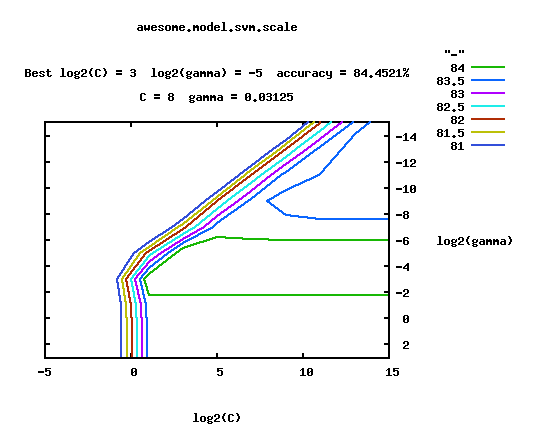
\includegraphics[width=1\columnwidth]{figures/parameter-selection.png}
\end{center}
\caption{An illustration of the grid search process to identify the best parameters values for training the SVM model.}
\label{fig:parameter_selection}
\end{figure}

\begin{itemize}

\item Grid search and grid search image

\item Include that PNG image from easy.py

\item Cross validation

\end{itemize}




\section{System}

\subsection{Code Architecture}

Include a system diagram of the code base.

Discuss and cite LIBSVM, LIBLINEAR and CRFSUITE.

\subsection{Web Service}

Where we can see the system running live.


\section{Results}

\subsection{Data Set}

Talk about the competition and where the data came from. How large the data size is, how much we trained on, etc.

\subsection{Trained Models}

Describe the different feature-subsets that we trained and why.


\subsection{System Performance}

How long each model took to train and how fast we can predict. Also discussion the hardware that was used to train and predict in terms of CPU speed, memory, etc.

\subsection{Evaluation}

A table of a bunch of awesome results. We should present results by model type (SVM, CRF, LIN) and feature set.

\subsection{Discussion}

Talk about what we saw in terms of which was the best feature set and model. 

Be sure to include examples of cool cases where it caught a difficult label

Be sure to include FAILURE cases

\section{Conclusion and Future Work}

I don't know, BS something...


\section{Acknowledgments}

We sincerely thank Dr. Robert Berwick  and Geza Kovacs
for their guidance, help, and support.


%%%% May the Flow (Max-Flow, that is) be with you all.

%
% The following two commands are all you need in the
% initial runs of your .tex file to
% produce the bibliography for the citations in your paper.
\bibliographystyle{abbrv}
\bibliography{citations}  % sigproc.bib is the name of the Bibliography in this case

\balancecolumns
% That's all folks!
\end{document}
